%%%%%%%%%%%%%%%%%%%%%%%%%%%%%%%%%%%%%%%%%%%%%%%%%%%%%%%%%%%%%%%%%%%%%%%%%%%%%%%%
%2345678901234567890123456789012345678901234567890123456789012345678901234567890
%        1         2         3         4         5         6         7         8

\documentclass[letterpaper, 10 pt, conference]{ieeeconf}  % Comment this line out if you need a4paper

%\documentclass[a4paper, 10pt, conference]{ieeeconf}      % Use this line for a4 paper

\IEEEoverridecommandlockouts                              % This command is only needed if 
                                                          % you want to use the \thanks command

\overrideIEEEmargins                                      % Needed to meet printer requirements.

% See the \addtolength command later in the file to balance the column lengths
% on the last page of the document

\makeatletter
\let\NAT@parse\undefined
\makeatother

\usepackage{xspace}
\usepackage{amsmath,amssymb,amsfonts,amsfonts}
\usepackage{algorithm}
\usepackage[noend]{algorithmic}
\usepackage{url}
\usepackage{bm}
\usepackage{graphicx,subfigure}
\usepackage{color}
\usepackage{hyperref}
%\hypersetup{bookmarksopen,
%bookmarksnumbered,
%pdfpagemode=UseOutlines,
%colorlinks=true,
%linkcolor=blue,
%anchorcolor=blue,
%citecolor=blue,
%filecolor=blue,
%menucolor=blue,
%urlcolor=blue
%}


\title{\LARGE \bf
Informed sampling by Markov Chain Monte Carlo methods
}


\author{
Rohan Thakker$^{*}$,
Cole Gulino$^{*}$,
Daqing Yi$^{}$,
Oren Salzman$^{}$ and
Siddhartha Srinivasa$^{}$% <-this % stops a space
\thanks{*R. Thakker and C. Gulino contributed equally to this paper.}
\thanks{This work was (partially) funded by the National Science Foundation IIS (\#1409003), Toyota Motor Engineering \& Manufacturing (TEMA), and the Office of Naval Research.}% <-this % stops a space
\thanks{$^{1}${\tt\small \{rthakker, cgulino, daqingy, osalzman, ss5\} @andrew.cmu.edu}}%
%
\\        
Robotics Institute, Carnegie Mellon University$^{1}$
}

%%%%%%%%%%%%%%%%%%%%%%%%%%%%%%%%%%%%%%%%%%%%%%%%%%%%%%%%%%%%%%%%%%%%%%%%%%%%%%
%  macros 
%%%%%%%%%%%%%%%%%%%%%%%%%%%%%%%%%%%%%%%%%%%%%%%%%%%%%%%%%%%%%%%%%%%%%%%%%%%%%%

% Caligraphic letters:
\newcommand{\calA}{\ensuremath{\mathcal{A}}\xspace}
\newcommand{\calC}{\ensuremath{\mathcal{C}}\xspace}
\newcommand{\calE}{\ensuremath{\mathcal{E}}\xspace}
\newcommand{\calG}{\ensuremath{\mathcal{G}}\xspace}
\newcommand{\calR}{\ensuremath{\mathcal{R}}\xspace}
\newcommand{\calM}{\ensuremath{\mathcal{M}}\xspace}
\newcommand{\calX}{\ensuremath{\mathcal{X}}\xspace}
\newcommand{\calS}{\ensuremath{\mathcal{S}}\xspace}
\newcommand{\calQ}{\ensuremath{\mathcal{Q}}\xspace}
\newcommand{\calT}{\ensuremath{\mathcal{T}}\xspace}
\newcommand{\calL}{\ensuremath{\mathcal{L}}\xspace}
\newcommand{\calB}{\ensuremath{\mathcal{B}}\xspace}
\newcommand{\calO}{\ensuremath{\mathcal{O}}\xspace}
\newcommand{\calP}{\ensuremath{\mathcal{P}}\xspace}
\newcommand{\calU}{\ensuremath{\mathcal{U}}\xspace}

% math
\newcommand{\R}{\mathbb{R}}
\newcommand{\Z}{\mathbb{Z}}
\newcommand{\A}{\mathbb{A}}
\newcommand{\N}{\mathbb{N}}
\newcommand{\Q}{\mathbb{Q}}
\newcommand{\C}{\mathbb{C}}
\newcommand{\K}{\mathbb{K}}
\newcommand{\D}{\mathbb{D}}


% Motion planning
\newcommand{\Cfree}{\ensuremath{\calX_{\rm free}}\xspace}
\newcommand{\Cforb}{\ensuremath{\calX_{\rm obs}}\xspace}
%\newcommand{\Cinf}{\ensuremath{\calX_{\hat{f}}}\xspace}
\newcommand{\Cinf}{\ensuremath{\calX_{\rm {inf}}}\xspace}
\newcommand{\Ufree}{\ensuremath{\calU_{\rm free}}\xspace}
\newcommand{\Pinf}{\ensuremath{\pi_{\hat{f}}}\xspace}


\newcommand{\Cbest}{\ensuremath{c_{\rm{curr}}}\xspace}

\newcommand{\Cs}{C-space\xspace}
\newcommand{\Css}{C-spaces\xspace}

\newcommand{\DOF}{\textit{dof}\xspace}
\newcommand{\DOFs}{\textit{dofs}\xspace}

\newcommand{\cbest}{\ensuremath{c_{\rm best}}\xspace}

% =
\newcommand{\eg}{{e.g.}\xspace}
\newcommand{\ie}{{i.e.}\xspace}
\newcommand{\etc}{{etc.}\xspace}
\newcommand{\etal}{{et~al.}\xspace}

\def\naive{{na\"{\i}ve}\xspace}

\def\os#1{\textcolor{magenta}{#1}}
\def\dy#1{\textcolor{cyan}{#1}}
\def\rt#1{\textcolor{green}{#1}}
\def\cg#1{\textcolor{blue}{#1}}
\def\ss#1{\textcolor{red}{#1}}

\def\deprecated#1{\vspace{3mm} \textcolor{red}{#1}  \vspace{3mm}}


\newtheorem{thm}{Theorem}
\newtheorem{lem}{Lemma}
\newtheorem{defn}{Definition}
%\newtheorem{thm}{Theorem}[section]
\newtheorem{observation}[thm]{Observation}
%\newtheorem{thm}{Theorem}
%\newtheorem{cor}[thm]{Corollary}
%\newtheorem{lem}[thm]{Lemma}


%tex tools
\newcommand{\ignore}[1]{}
\newcommand{\first}[2]{#1}
\newcommand{\second}[2]{#2}
\newcommand{\arxiv}[2]{#2}



\newcommand{\captionstyle}{\sf \footnotesize }

\renewcommand\algorithmiccomment[1]{%
  \hfill\#\ \eqparbox{COMMENT}{#1}%
}

\begin{document}

\maketitle
\thispagestyle{empty}
\pagestyle{empty}


%%%%%%%%%%%%%%%%%%%%%%%%%%%%%%%%%%%%%%%%%%%%%%%%%%%%%%%%%%%%%%%%%%%%%%%%%%%%%%%%
\begin{abstract}

\end{abstract}


%%%%%%%%%%%%%%%%%%%%%%%%%%%%%%%%%%%%%%%%%%%%%%%%%%%%%%%%%%%%%%%%%%%%%%%%%%%%%%%%
\section{Introduction}
\label{sec:intro}


Sampling-based motion-planning algorithms~\cite{CBHKKLT05, L06} have proven to be an effective tool at solving motion-planning problems.
They search through a continuous state space~$\calX$ by sampling random states and maintaining a discrete graph~$G$ called a \emph{roadmap}.
Vertices and edges in $G$ correspond to collision-free states and paths, respectively.

Roughly speaking, these algorithms iteratively sample new states.
This is required to ensure that, as the number of samples tends to infinity, 
(i)~a solution will be found 
(a property called \emph{probabilistic completeness})
and that
(ii)~given some optimization criteria, the quality of the solution will progressively converge to the quality of the optimal solution
(a property called \emph{asymptotic  optimality}).

Initially, 
when a path has yet to be found, 
the samples need to be drawn from the entire state space~$\calX$.
However, once a path $\gamma$ is produced,  algorithms that seek \emph{high-quality paths} can limit their sampling domain to a subset of~$\calX$ only  containing states that may produce higher-quality paths than~$\gamma$.
Following Gammell et al.~\cite{GSB14}, we call this subset the \emph{informed subset} and denote it~$\Cinf$.
\textbf{In this work we address the problem of efficiently producing samples in informed subset for systems with differential constraints}. 

For Euclidean spaces optimizing for path length, 
\Cinf can be analytically expressed as a prolate hyperspheroid and can be sampled directly using a closed form solution~\cite{GSB14}.
Indeed, directly sampling in \Cinf has been shown to dramatically improve computation time when compared to sampling in $\calX$, especially in high dimensions. 

Unfortunately, in more general settings such as
for systems with differential constraints,
it is not clear how to directly sample \Cinf.
%
One approach to produce samples in \Cinf is via \emph{rejection sampling}---sampling a state $x \in \calX$ and testing if $x \in \Cinf$.
However, when the size of the informed space~$\Cinf$ is much smaller than entire state space~$\calX$, then this procedure may dominate the running time of the algorithm~\cite{KTC16}.
Recently, Kunz et al.~\cite{KTC16} showed, under some technical assumptions, how to efficiently produce samples in~$\Cinf$ by \emph{Hierarchical rejection sampling} (HRS). 
Here, individual dimensions are sampled recursively 
and then combined. Rejection sampling is performed for these partial samples until a suitable sample has been produced. 
%The novelty of HRS is the ability to fail fast. 

Unfortunately, both rejection sampling and HRS may produce a large number of rejected samples especially in high-dimensional spaces.
This may cause the search algorithm to spend most of its time trying to produces samples in~$\Cinf$ rather than explore it.
In this paper, we suggest an alternative approach to produce samples in the informed set \Cinf for a wide range of settings.
\textbf{Our main insight is to formulate the problem as the problem of sampling uniformly below a level set of an implicit function and then apply optimization and statistical tools.}
Specifically, our approach consists of two stages:
in the first, a random sample $x \in \calX$ is retracted to the boundary of~$\Cinf$ by running a gradient-descent algorithm;
in the second stage, this retracted sample $\tilde{x}$ is used to seed a Monte Carlo sampling chain which allows us to  produce samples that (approximately) cover~$\Cinf$  uniformly.

Our approach requires that the system has a solution to the two-point boundary value problem (2pBVP)~\cite{L06, H02} and that a gradient can be defined over the cost function.
Indeed, we demonstrate the efficiency of our approach on a wide variety of systems and show that it enables reducing the planning time by several orders of magnitute when compared to algorithms using rejection sampling or HRS.

%While, original sampling-based algorithms such as RRT~\cite{LK01} and PRM~\cite{KSLO96} only guaranteed to asymptotically return \emph{a} solution, if one exists, they did not provide any guarantees on the \emph{quality} of the solution, given some optimization criteria.
%Karaman and Frazzoli~\cite{KF11}, presented variants of PRM and RRT, named PRM* and RRT*, respectively that were shown to produce paths who's cost converges asymptotically to the minimal-cost path.
%Additional algorithms followed, increasing the converges rate by various techniques such as lazy dynamic programming~\cite{GSB15, JSCP15}, relaxing optimality to near-optimality~\cite{DB14, SH16} and more.
%
%However, recent years 
%Original planners such as RRT~\cite{LK01} and PRM~\cite{KSLO96} did not provide any guarantee on the \emph{s}


\section{Related work}
\label{sec:related_work}
We start in Sec.~\ref{subsec:planning} by giving an overview of relevant sampling-based motion-planning algorithms.
We then continue in Sec.~\ref{subsec:sampling} to describe different approaches used to sample~$\calX$.
We conclude our literature review in Sec.~\ref{subsec:mcmc} with a brief overview of Markov Chain Monte Carlo methods.

\subsection{Planning}
\label{subsec:planning}
Initial sampling-based algorithms such as RRT~\cite{LK01} and PRM~\cite{KSLO96} did not take into account the \emph{quality} of a path, given some optimization criteria, and only guaranteed to asymptotically return \emph{a} solution, if one exists.
Karaman and Frazzoli~\cite{KF11}, presented variants of PRM and RRT, named PRM* and RRT*, respectively that were shown to produce paths who's cost converges asymptotically to the minimal-cost path.
This is done by recognizing the underlying connections between stochastic sampling-based motion planning and the theory of random geometric graphs (see also~\cite{SSH16}).
Additional algorithms followed, increasing the converges rate by various techniques such as lazy dynamic programming~\cite{GSB15, JSCP15}, relaxing optimality to near-optimality~\cite{DB14, SH16} and more.


Many of the algorithms mentioned require solving a two-point boundary value problem (2pBVP) to perform exact and optimal connections between vertices in the roadmap.
For holonomic robots, these are simply straight lines in the state space, but for kinodynamic sytems with arbitrary cost functions,  computing an optimal trajectory between two states is non-trivial in general.

Xie et al.~\cite{XBPA15} use a variant of sequential quadratic programming (SQP) to solve 2pBVP and integrate it with BIT*~\cite{GSB15}.
Webb and van den Berg~\cite{WB13} use a fixed-final-state-free-final-time controller to solve the 2pBVP  with respect to a cost function that allows for balancing between the duration of the trajectory and the expended control effort.
Perez et al.~\cite{PPKKL12} propose a variant of RRT* that automatically defines a distance metric and node extension method by locally linearizing
the domain dynamics and applying linear quadratic regulation (LQR).

%Finally, we note that there have been many papers presenting solutions to the 2pBVP for specific systems such as
%
%Jeong Hwan Jeon, Raghvendra V. Cowlagi, Steven C. Peters, Sertac Karaman, Emilio Frazzoli, Panagiotis Tsiotras, Karl Iagnemma: Optimal motion planning with the half-car dynamical model for autonomous high-speed driving. ACC 2013: 188-193
%Dubins cars optimizng for both time and energy (RSS submission 107 by Shammas, Elie) 

%possible additional papers on Kinodynamic RRT*:~\cite{KF10, GPPK13}

\subsection{Sampling}
\label{subsec:sampling}
There is a rich body of literature on how to produce samples that increase the efficiency of the planner in terms of finding a solution or producing high-quality solutions.
Heuristic approaches include
sampling on the medial axis~\cite{WAS99a, WAS99b, LTA03, YDLTA14},
sampling near the boundary of the obstacles~\cite{ABDJV98, YTEA12},
resampling along a given trajectory~\cite{APD11, AS11}
and more~\cite{US03, SWT09}

Of specific interest to our work are approaches that produce samples in the informed set~\Cinf.
As mentioned in Sec.~\ref{sec:intro} Gammel et al.~\cite{GSB14} describe an approach to sample uniformly in~\Cinf for the specific case of where $\calX = \R^d$ and when optimizing for path length.
To the best of our knowledge, the only method to produce samples in non-Euclidean spaces (other than rejection sampling) is HRS by Kunz et al.~\cite{KTC16}.

\subsection{MCMC}
\label{subsec:mcmc}

An alternative sampling framework, which is widely used in statistical machine learning, is Monte Carlo Simulation~\cite{M97}.
It uses the numerical experimental power of computers to generate samples toward a desired distribution $ \pi (x) $.
The generated set of samples are a discrete approximation $ \hat{\pi} (x) $ of the desired distribution $ \pi (x) $.
A approximated desired distribution $ \hat{\pi} (x) $ can be used in any problem that states are modeled random variable, e.g. motion tracking~\cite{KBD04}, data regression~\cite{TL11} and state estimation~\cite{ASC13}.

Markov Chain Monte Carlo (MCMC)~\cite{ADDJ03} is one most popular class that constructs a Markov chain of random transition that moves samples from an original proposed distribution to a desired distribution $ \pi (x) $.
The random movement is driven by a jumping distribution $ g(x' \mid x) $, which samples a new state $ x' $ by a given state $ x $.
The idea of MCMC is designing a jumping distribution $ g $ that makes the desired distribution a stationary distribution $ \pi = \pi * g $.
\emph{Ergodic theorem} shows that if the jumping distribution is aperiodic, irreducible and positive recurrent~\cite{AG11}, samples generated from arbitrary distributions will gradually converge to the stationary (desired) distribution $ \pi $.
In practice, samples are initially generated from an arbitrary distribution.
They shall converge to the samples generated from the desired distribution () 
A few MCMC algorithms, e.g. Gibbs sampling and Metropolis-Hastings, have been widely used in sampling from distributions that are difficult to directly sample.

The nature of random walk in MCMC sometimes requires too many iterations to converge, especially in high-dimension state spaces.
In consider of efficiency, Hamiltonian Monte Carlo(HMC)~\cite{N11} is thus introduced to replace random walk with Hamiltonian dynamics, which means that future states in the Markov chain is proposed from simulating system dynamics instead of sampling from a jumping distribution.
It is named ``Hamiltonian, because the concept origins from Hamiltonian dynamics, which defines how system dynamics is determined by system energy.
Define the system dynamics of an object as the position $ x $ and the momentum $ q $ over time $ t $.
We have a system energy $ H $ of the object that consists of kinetic energy $ K $ and potential energy $ U $, which is written as $ H(x,q) = U(x) + K(q) $.
The kinetic energy $ K(q) $ is determined by the momentum $ q $ of the object, while the potential energy $ U(x) $ is determined by the position $ x $ of the object.
The Hamiltonian dynamics is determined by the gradients of the system energy, which is
$ \frac{dx}{dt} = \frac{\partial H}{\partial q} $ and $ \frac{dq}{dt} = - \frac{\partial H}{\partial x} $.

The canonical distribution is often choose to bridge a system energy with a probability distribution, which is written as $ P(x, q) = \frac{1}{Z} \exp ( -H(x,q) / T ) $.
If two different states have the same energy, the probabilities of them are equivalent.
It has been proved that properties of Hamiltonian dynamics ``leaves the canonical distribution invariant"~\cite{N11}, which means $ P(x, q) $ equals to a stationary distribution in MCMC.
Thus, we can generate samples $ [ x , q ]^T $ from joint distribution $ p(x, q) $.

Given a target distribution $ \pi(x) $, the potential energy is defined in the form $  U(x) = - \log ( \pi(x) T ) $.
We can have $ P(x, q) = \pi(x) \frac{1}{Z'} \exp ( -K(q) / T ) $, which indicates that $ pi(x) $ is a marginal distribution of $ P(x, q) $.
In HMC, we sample $ [ x ,q ] $ from $ P(x, q) $ and discard the momentum $ q $ so that the set of samples $ x $ equals to sampling from the marginal distribution $ \pi(x) $.
The momentum $ q $ is used as an auxiliary variable.
Avoiding random walk helps samplings converge to the desired distribution $ \pi(x) $ in higher rate~\cite{N11}.



\section{Motivating example---Minimal-Time Double Integrator}

We start by considering a simple yet important dynamical system---the double integrator. 
We are given a one-dimensional point robot with bounded velocity and bounded acceleration moving amid obstacles. We wish to compute the minimal-time trajectory between two states $x_s, x_g$.
A state in this model is described by 
the position $q \in \R$
and
the velocity $\dot{q}\in \R$ of the position.
%each coordinate axis.
The dynamics of the system is described by:

\begin{equation}
x = (q, \dot{q}); 
\hspace{5mm}
u = \ddot{q}.
\end{equation}

Here, the control $u \in [u_{\text{min}}, u_{\text{max}}]$ is the (bounded) acceleration. 


Notice that 
(i)~this is model can be seen as a simplified one-dimensional instance of a robot manipulator with many degrees of freedom and that
(ii)~closed form solutions exist to the 2pBVP for this specific case (as well as the generalized instance)~\cite{HN10}.

Let $T(x_1, x_2)$ denote the minimal time to move the robot from state $x_1$ to $x_2$.

Further, set
\begin{equation}
T(x) = T(x_s, x) + T(x, x_g).
\end{equation}

Namely, $T(x)$ is the minimal time to reach the goal from the start subject to passing through the state $x$.

\subsection{Informed set}
Recall that for Euclidean spaces minimizing path length, the informed set is a prolate hyperspheroid.
Moreover, this ellipsoid is defined only be the cost $\hat{c}$ of the current best solution and not by the location of the start and goal.

For the case of a double integrator, this is not the case. Intuitively, one can see why. According the the double-integrator minimum time model, maximum acceleration is applied in one direction to a point, and then maximum acceleration in the other direction is applied to complete the motion. The direction of the first and second acceleration depends on the start and goal state.

See Fig. ~\ref{fig:sample_dimt} for an example motion of one joint through the $\left(x,\dot{x}\right)$ space. 

\begin{figure}[tb]
  \centering
  	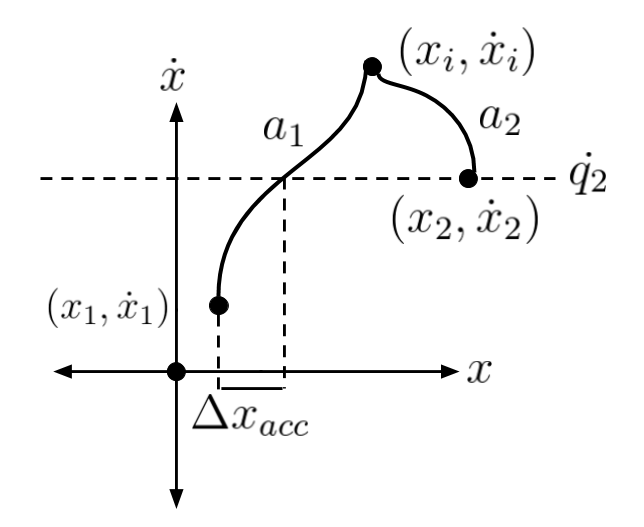
\includegraphics[width=0.3\textwidth]{fig/example_motion.png}
  \caption{
    \captionstyle
  	Example possible motion using the double-integrator minimum time model between start state $(x_1, \dot{x_1}$ and goal state $(x_2, \dot{x_2}$ through some intermediate state $(x_i, \dot{x_i})$.
  	}
   	\label{fig:sample_dimt}
\end{figure}

In order to find the minimum time, $T\left(x\right)$, of a motion like Fig. ~\ref{fig:sample_dimt}, we can examine the paths separately with one corresponding to a motion with acceleration $a_1$ from $\left(x_1, \dot{x}_1\right)$ to $\left(x_i, \dot{x}_i\right)$ and another corresponding to motion with acceleration $a_2$ from $\left(x_i, \dot{x}_i\right)$ to $\left(x_2, \dot{x}_2\right)$.

\ref{} shows that we can express total distance travelled in the joint space $x$ can be expressed in this way as:

\begin{equation}
x_2 - x_1 = d_{a_1} + d_{a_2}
\end{equation}
where $d_{a_1}$ is the distance travelled at max acceleration from the first path and $d_{a_2}$ is the distance travelled at max acceleration in the opposite direction.

Using simple constant acceleration equations we can express this in the form:

\begin{equation}
x_2 - x_1 = \left(\dot{x}_1 t_{a_1} + \frac{1}{2} a_1 t_{a_1}^2\right) + \left(\frac{\dot{x}_2^2 - \dot{x}_i^2}{2a_2}\right)
\end{equation}
where $t_{a_1}$ is the time it takes to make the path from $\left(x_1, \dot{x}_1\right)$ to $\left(x_i, \dot{x}_i\right)$ at acceleration $a_1$ and $t_{a_2}$ is the time it takes to make the path from $\left(x_i, \dot{x_i}\right)$ to $\left(x_2, \dot{x}_2\right)$ at acceleration $a_2$.

We can further expand the equation in order to put it into the canonical quadratic equation as follows:

\begin{equation}
a_1 t_{a_1}^2 + 2 \dot{x}_1 t_{a_1} + \frac{\dot{x}_2^2 - \dot{x}_1^2}{2a_2} - \left(x_2 - x_1\right) = 0
\end{equation}

Following ~\ref{} we solve a quadratic equation of the form $at^2+bt+c=0$ as follows:

$$
q = -\frac{1}{2}\left(b + \text{sign}\left(b\right)\sqrt{b^2 - 4ac}\right)
$$
$$
t_1 = \frac{q}{a}; \hspace{5mm} t_2 = \frac{c}{q}
$$
where $t_1$ and $t_2$ are the two solutions to the quadratic equation.

As we know, time must be positive and we are looking for minimum time. This leads to the fact that there is only one correct solution to the quadratic equation. Because of this, depending on the start and goal states, the sign of the acceleration on each path will change.

Again following ~\ref{}, we programatically solve for the sign of the sign of the acceleration by analysing the start and goal position. Fig. ~\ref{fig:sample_dimt} shows the determining term $\Delta x_{acc}$, which is the distance from $x_1$ to the point where $\dot{x} = \dot{x}_2$. 

And using constant acceleration equations with ~\ref{} again, we find that:

\begin{equation}
\Delta x_{acc} = \frac{1}{2} \left(\dot{x}_1 + \dot{x}_2\right) \frac{|\dot{x}_2 - \dot{x}_1|}{a_{max}}
\end{equation}

\begin{equation}
a_1 = - a_2 = \text{sign}\left(x_2 - x_2 - \Delta x_{acc}\right) a_{max}
\end{equation}

From these equations it shows a fundamental difference of a kinodynamic state space compared to a geometric state space. Because of this the minimum time path can vary in shape depending on the start and goal state. The consequence of this is that the shape of the informed subset can change dramatically depending on the start and goal state of the problem definition. Because of this, finding a closed form solution to sampling in the informed space is not feasible.

See Fig.~\ref{fig:informed_1d_di} for a visualization of the cost surface for a specific start and goal state for one degree of freedom (two dimensions $\left(x, \dot{x}\right)$). Lower costs are represented with cooler colors with warmer colors representing higher costs. One can see the minimum cost path from start to goal as the dark blue curve.

\begin{figure}[tb]
  \centering
  	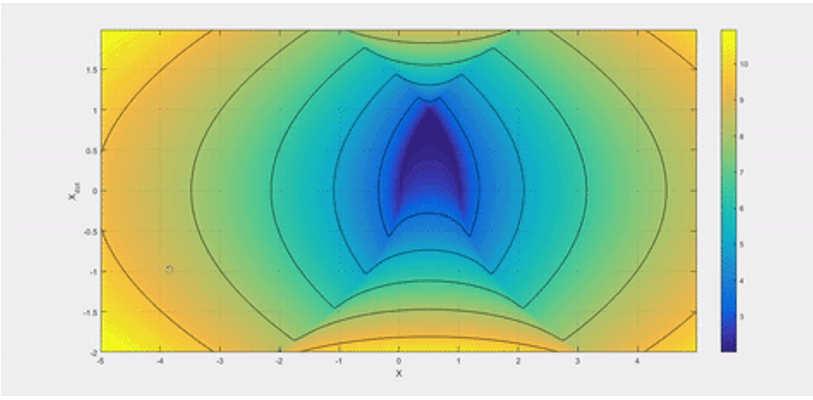
\includegraphics[height = 4.cm ]{fig/level_set.jpg}
  \caption{
    \captionstyle
  	Level sets for the case of minimal-time double integrator. A point $x = (q, \dot{q})$  denote the position and velocity of the robot while the color at $x$ denotes the cost to reach $x_t$ from $x_s$ subject to passing through the state $x$.
  	}
   	\label{fig:informed_1d_di}
	\vspace{-5.5mm}
\end{figure}

\begin{figure}[tb]
  \centering
  	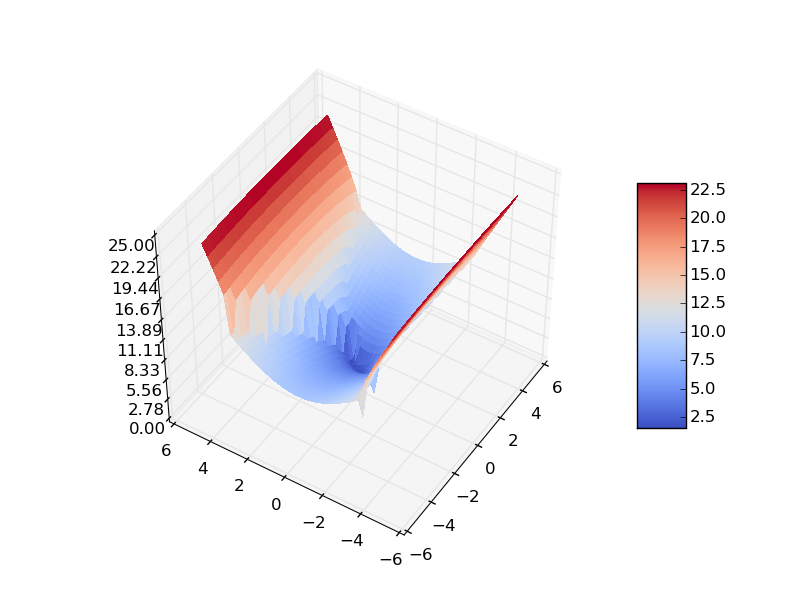
\includegraphics[width=0.5\textwidth]{fig/kino_space.png}
  \caption{
    \captionstyle
  	Side view of the cost surface for the case of minimal-time double integrator. The side view showcases the discontinuous nature of the cost surface.
  	}
   	\label{fig:cost_surface_1d}
	\vspace{-5.5mm}
\end{figure}

See Fig. ~\ref{fig:cost_surface_1d} for a side view of the cost surface for one degree of freedom ($\left(x, \dot{x}\right)$). One can see a key property of the cost surface that cause serious concerns is the discontinuous nature of the surface. As mentioned before, finding the minimum time problem amounts to solving a quadratic equation. Because the nature of this equation changes with the start and end goal, there is a curve in the input space that amounts to a switching surface that represents the boundary for the decision of the sign of $a_1$. This surface causes a discontinuous cost surface as shown in Fig. ~\ref{fig:cost_surface_1d}.


\section{Algorithm}
\label{sec:algorithm}

Define the dynamics of a robot as 
\begin{equation}
\label{eq:kinematics}
\dot{\bm{x}}(t) = f( \bm{x}(t) , \bm{u}(t) ), 
\end{equation}
in which $ \bm{x} \in \mathcal{X} \subseteq \mathbb{R}^n $ is the state of the robot, and $ \bm{u} \in \mathcal{U} \subseteq \mathbb{R}^m $ is the control input.
The dynamics determines a state trajectory $ \pi $, given a duration $ T $, an initial state $ \bm{x}(0) $ and an initial input $ \bm{u}(0) $.
The cost of a trajectory $ \pi $ is defined as the accumulated cost along the path, which is 
\begin{equation}
\label{eq:path_cost}
c(\pi) = \int_0^{T} c( x(t), u(t) ) dt.
\end{equation}
Consider the obstacles in a workspace, we have $ \mathcal{X}_{free} \subseteq \mathcal{X} $.
Consider the bounds of the control input, we have $ \mathcal{U}_{free} \subseteq \mathcal{U} $.
The dynamics of the robot in Equation~\eqref{eq:kinematics}, free state space $  \mathcal{X}_{free} $ and free control input space $ \mathcal{U}_{free} $ determines a free trajectory space $ \Pi_{free} $, which contains all feasible trajectories $ \pi \in \Pi_{free} $.

We can define an optimal kinodynamic path-planning problem that finds a kinodynamic path minimizing the cost in Definition \ref{defn:optimal_kino_path_planning}.
\begin{defn}{ \textbf{Optimal Kinodynamic Path-Planning} }
\label{defn:optimal_kino_path_planning}
	Find an optimal path $  \pi^* $ that satisfies
	\begin{itemize}
	\item $\forall t \in [0,T] $, $ \bm{x} (t) \in \mathcal{X}_{free}  $ and $ \bm{u} (t) \in \mathcal{U}_{free} $;
	\item $ \bm{x} (0) = x_{init} $, $ \bm{x} (T) = x_{goal} $, $ \bm{u} (0) = u_{init} $ and $ \bm{u} (T) = u_{goal} $; and
	\item $ \pi^* = \max_{ \pi \in \Pi_{free} } c( \pi ) $. 
	\end{itemize}
\end{defn}

\dy{Do we want to set an initial and a goal for the control input? Does this simplify the problem solving?}

\dy{I am not sure what we want to put into here, but I am going to continue on the discussion of the algorithm and talk about some of the probability stuff.}

One of the major difficulties of sampling the informed level set is that the shape of the cost function can change dramatically with the start and goal states. Because of this, there is not a principled way to sample from the informed set for each possible start and goal combination.  

Following the example of recent work in path planning algorithms such as ~\ref{} (CHOMP?), we propose to solve the problem of efficiently sampling uniformly in the level set by using Monte Carlo sampling methods. Monte Carlo sampling methods have been used in the statics and machine learning fields to sample from intractable posteriors. Monte Carlo methods have the desirable property that they are guaranteed to sample the true posterior as the number of steps goes toward infinity.

In order to take advantage of these powerful methods, we propose to reformulate the cost surface as a probability density. Specifically, we consider a Boltzmann distribution in order to formulate the cost function using flexible energy based methods. Because Monte Carlo methods only consider the ratio of the probabilities, we do not need to consider the problem of estimating the intractable partition function.

Formally, we consider the probability distribution to be a Boltzmann distribution in the form of:

\begin{equation}
P\left(t,t_0\right) = \frac{1}{Z}\exp\left(-E\left(t,t_0\right)\right)
\end{equation}
where $Z$ is the intractable partition function that denotes the normalizing constant of the distribution and  $E\left(t,t_0\right)$ is the energy function which is dependent on the current best cost, $t_0$, and the cost of the path in question $t$.

The flexibility of the energy function is in the ability to specify desired or more probable states (by presenting lower energies) without the need to use a formal and restrictive model. Specifically for our problem, we defined the energy function to be:

\begin{equation}
E\left(t, t_0\right) = E_{\text{grad}}\left(t\right) + E_{\text{informed}}\left(t,t_0\right) + E_{\text{region}}\left(\mathbf{x}\right)
\end{equation}

\begin{equation}
E_{\text{grad}}\left(t\right) = \sigma\left(t\right)
\end{equation}
where $\sigma\left(\cdot\right)$ is some function that controls the flatness of the distribution.  Intuitively, this function prefers states with smaller costs. The flatter the function, the less pronounced this becomes. We experimented with using $\log\left(1 + \log\left(t\right)\right)$ and $\tanh\left(t\right)$. $\tanh$ resorts in a flatter distribution which may result in more uniform samples, but contains less gradient information for methods that use them such as Hamiltonian Monte Carlo.

\begin{equation}
E_{\text{informed}}\left(t,t_0\right) = \beta_{\text{informed}} \text{sigm}\left(t_0 - t\right)
\end{equation}
where $\text{sigm}\left(\cdot\right)$ represents a tight sigmoid function that can be seen as a differentiable $\text{sign}\left(\cdot\right)$ function. $\beta_{\text{informed}}$ is some large number that controls how much we want to penalize states outside of the level set. In theory, the energy should be infinity (which represents zero probability). In practice, however, setting $\beta_{\text{informed}}$ to be some high number such as $100$ works well and is more stable.

\begin{equation}
E_{\text{region}}\left(\mathbf{x}\right) = \beta_{\text{region}}||\mathbf{x}_{\text{limits}} - \mathbf{x}||_2
\end{equation}
where $||\mathbf{x}_{\text{limits}} - \mathbf{x}||_2$ represents the L2 distance between the current state $\mathbf{x}$ and the state limits $\mathbf{x}_{\text{limits}}$ and $\beta_{\text{region}}$ is some high number that controls how much to penalize states close to the limits. The same intuition for values of $\beta_{\text{region}}$ is the same as for $\beta_{\text{informed}}$.

In order to ensure that the span the set of all possible states 

\begin{algorithm}
	\begin{algorithmic}[1]
		\STATE
   	\end{algorithmic}
	\caption{MCMC Informed Sampling}
	\label{alg:mcmc_informed_sampling}
\end{algorithm}


\section{Results}

\subsection{Uniformity}

(Give a set of parameters)
We firstly need to propose a way of measuring uniformity.
Then we can apply it to compare MCMC approach with rejection sampling and hierarchical rejection sampling.
We are interested with
\begin{itemize}
	\item asymptotic behavior (assumption: MCMC converge to a close uniformity)
	\item convergence rate (assumption: MCMC converge faster)
\end{itemize}

\subsection{Efficiency}

The efficiency is shown by how the time is needed when the number of nodes are increased.
(Y: time spent) and (X: number of nodes).

\subsection{Integration}

We're going to test with RRT*, which falls into a informed RRT*.

We are going to show how the solution cost falls along time.
(Y: solution cost) and (X: time spent).

\begin{itemize}
\item DIMT (double integrator minimum time)
\item Dubins car
\item Airplane
\end{itemize}

\section{Conclusion}





%%%%%%%%%%%%%%%%%%%%%%%%%%%%%%%%%%%%%%%%%%%%%%%%%%%%%%%%%%%%%%%%%%%%%%%%%%%%%%%%

\bibliography{bibliography}
\bibliographystyle{IEEEtran}
%\bibliography{IEEEabrv,bibliography}


\end{document}
